\documentclass{article}
\usepackage[italian]{babel}
\usepackage{hyperref}
\usepackage{graphicx}
\usepackage{float}
\usepackage[x11names,table]{xcolor}
\usepackage{array}
\graphicspath{ {./imgs/} }

\title{VezGammon - Report finale Team 1 \\ \large Progetto di Ingegneria del Software}
\author{Lorenzo Peronese - Scrum Master}

\begin{document}

\maketitle

\tableofcontents

\newpage

\section{Descrizione del prodotto}
\subsection{Introduzione}
Per il progetto del corso di Ingegneria del Software, il team ha scelto di lavorare a VezGammon\textsuperscript{\texttrademark}, 
un'applicazione web di backgammon. Il progetto ha diversi riferimenti alla città di Bologna, in cui è nato e si è sviluppato: 
in primis ovviamente il nome (\textit{"vez"} viene usato a Bologna come intercalare e significa amico, fratello); inoltre una 
volta nel sito il cursore diventa un simpatico tortellino e la board utilizza i colori rosso e blu, rappresentativi della città.

L'applicazione offre un'esperienza di gioco completa con diverse modalità: gli utenti possono sfidarsi in partite locali sullo 
stesso dispositivo, mettere alla prova le proprie abilità contro intelligenze artificiali di vari livelli di difficoltà e confrontarsi 
online con altri giocatori attraverso un sistema di matchmaking o mediante link di invito diretti. È inoltre possibile organizzare 
tornei a quattro partecipanti, combinando liberamente giocatori reali e agenti intelligenti.

Il sistema di classificazione si basa sul metodo Elo, ampiamente utilizzato negli scacchi. Ogni nuovo account parte da una base 
di 800 punti, che vengono poi aggiornati dopo ogni partita online o torneo. Il calcolo dell'aggiornamento tiene conto di diversi 
fattori: l'esito della partita, l'utilizzo del dado double e il punteggio Elo di entrambi i giocatori. Questo sistema garantisce 
una competizione equilibrata e permette di mantenere una classifica globale, dove ogni giocatore può aspirare a raggiungere le 
posizioni più alte.

VezGammon\textsuperscript{\texttrademark} include anche ricche funzionalità social e di progressione. Gli utenti possono consultare 
(e condividere sui social) in ogni momento statistiche dettagliate delle proprie partite, visualizzare grafici che mostrano l'andamento 
del proprio Elo nel tempo e analizzare i match recenti. Il sistema premia inoltre i giocatori con speciali badge al raggiungimento 
di specifici obiettivi, come vincere un determinato numero di partite o raggiungere certi livelli di punteggio Elo, aggiungendo 
un ulteriore elemento di coinvolgimento e progressione al gioco.

\subsection{Backlog} \label{sec:bl}
\begin{figure}[H]
    \centering
    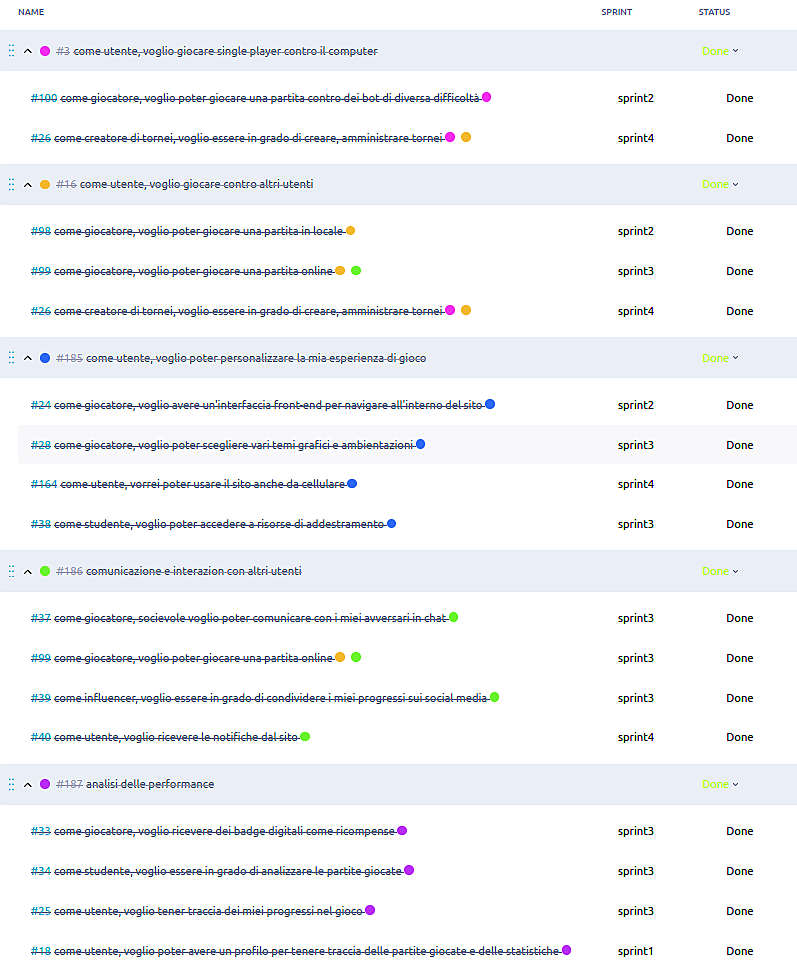
\includegraphics[width=12cm, height=14cm]{backlog}
    \caption{Backlog di Taiga di Vezgammon\textsuperscript{\texttrademark}}
    \label{fig:backlog}
\end{figure}

\subsection{UML}
\subsubsection{Casi d'uso}

\begin{figure}[H]
    \centering
    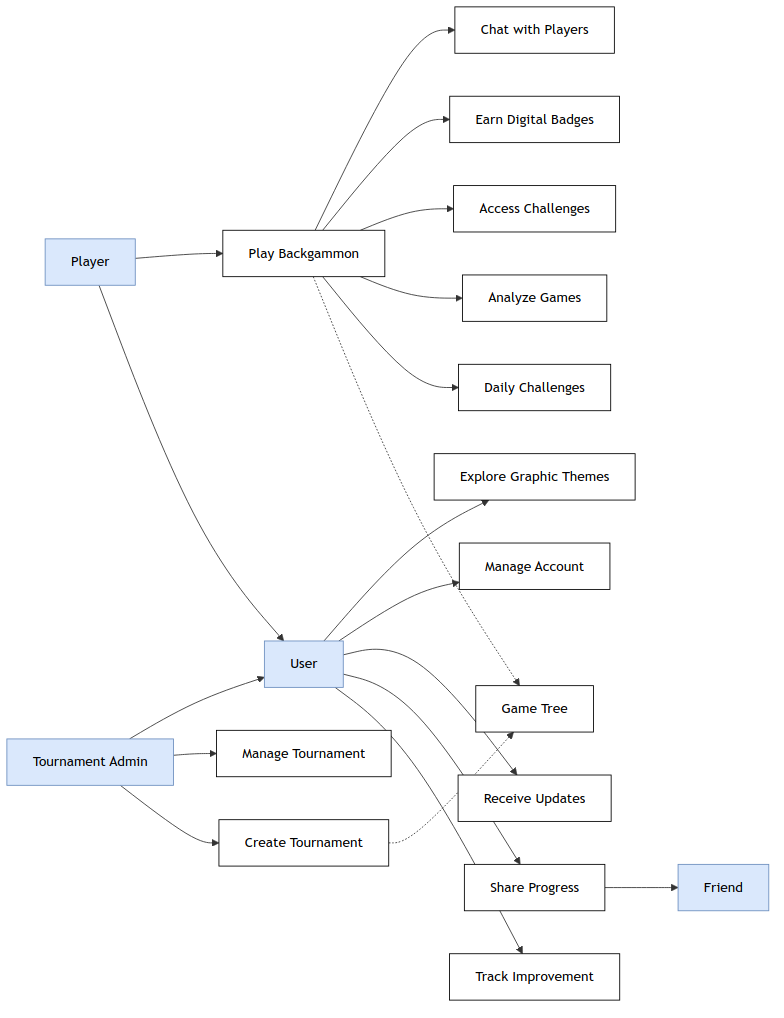
\includegraphics[width=12cm]{uml-usecase}
    \caption{Diagramma UML use-case}
    \label{fig:use-case}
\end{figure}

\subsubsection{Deployment}

\begin{figure}[H]
    \centering
    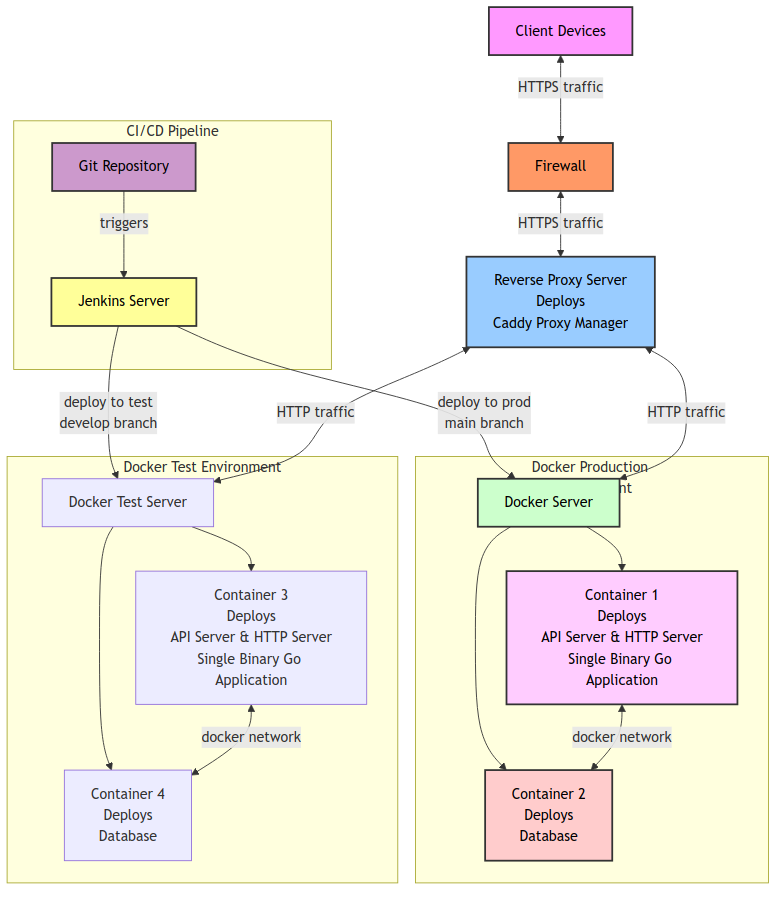
\includegraphics[width=12cm]{uml-deployment}
    \caption{Diagramma UML di deployment}
    \label{fig:deployment}
\end{figure}

\subsubsection{Classi}

\begin{figure}[H]
    \centering
    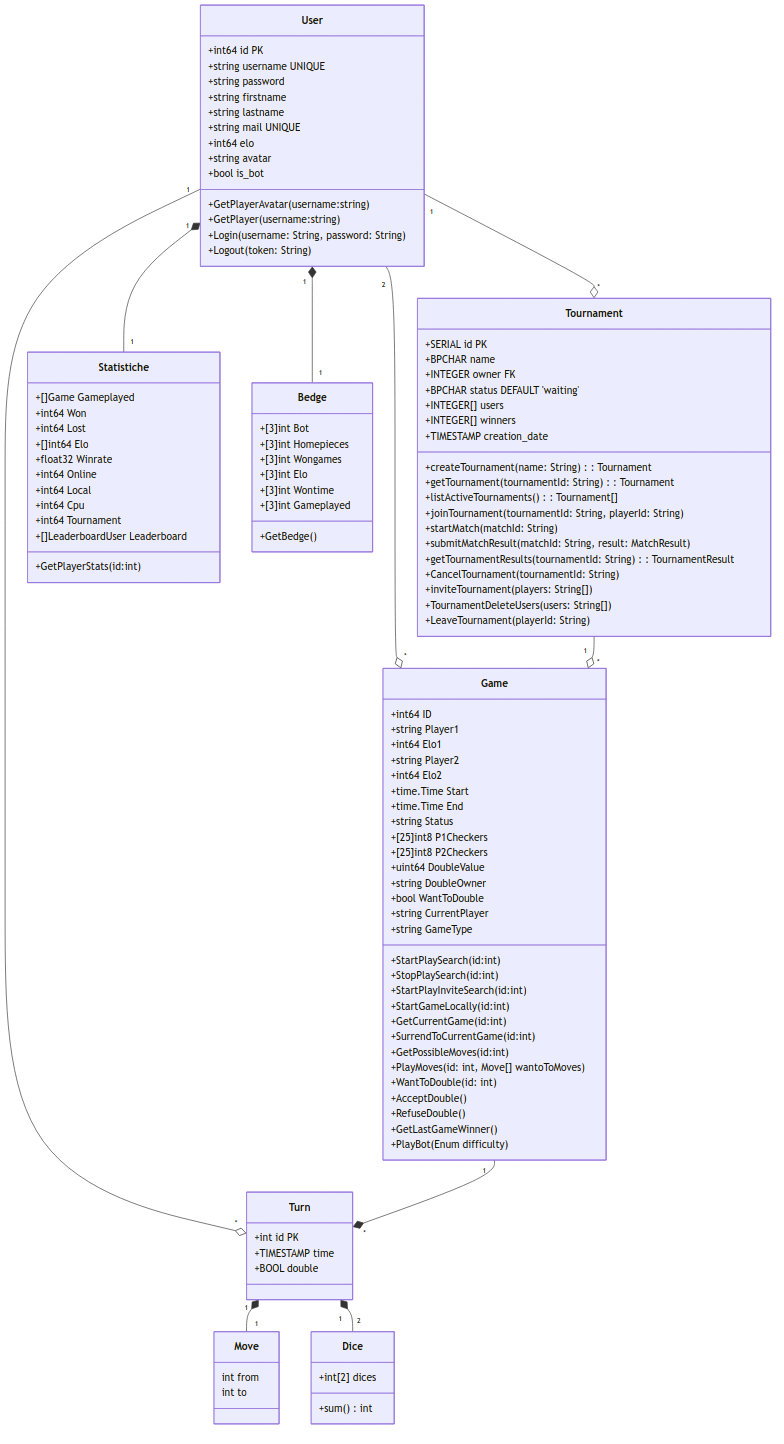
\includegraphics[width=12cm, width=8cm]{uml-classes}
    \caption{Diagramma UML delle classi}
    \label{fig:class-diagram}
\end{figure}

\subsubsection{Tornei}

\begin{figure}[H]
    \centering
    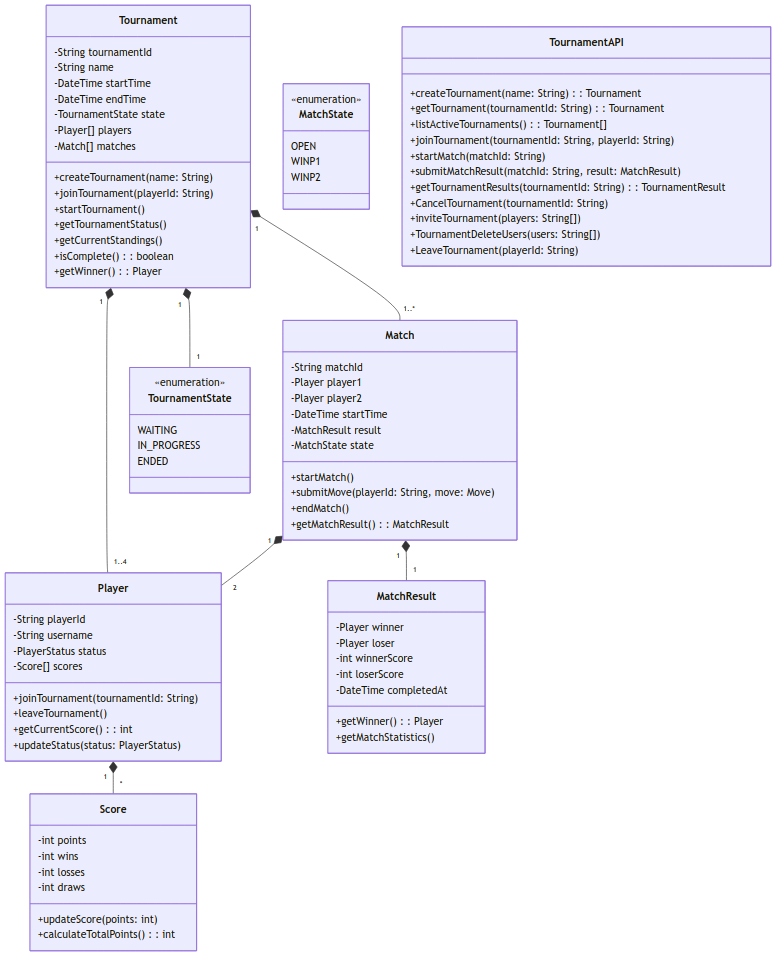
\includegraphics[width=12cm]{uml-tournaments}
    \caption{Diagramma UML dei tornei}
    \label{fig:tournaments}
\end{figure}

\section{Infrastruttura e software utilizzato}

\subsection{CAS: ambiente di sviluppo agile}

Il team ha adottato un approccio completamente open source, basandosi sull'ambiente CAS consigliato dai docenti. 
Tutti software sono stati self-hostati sotto il dominio \href{https://vezgammon.it}{\texttt{vezgammon.it}} per garantire 
un maggiore controllo e personalizzazionee avere meno dipendenze possibili con l'esterno. Questo ha inizialmente richiesto 
un notevole sforzo ma a lungo termine sono emersi i benefici di questa scelta.

Le credenziali di accesso sono state fornite agli stakeholder al momento della creazione dell'infrastruttura ma possono 
essere resettate su richiesta.

\subsubsection{GitLab}
GitLab è stato utilizzato per la gestione del codice sorgente e per il versioning. Sono stati utilizzati i tag per denotare 
il Minimun Value Product di ogni sprint. 
Il team ha qui configurato il repository, gestito le merge request e segnalato e risolto le issue.

Il repository è accessibile all'indirizzo \href{https://gitlab.vezgammon.it}{\texttt{gitlab.vezgammon.it}}  

\subsubsection{Taiga}
Taiga è stato scelto per la gestione del project management. È stato utilizzato per tracciare le attività, gestire il 
backlog (vedi \ref{sec:bl}), definire le user stories e monitorare lo stato di avanzamento del progetto durante gli sprint.

Il progetto Taiga è accessibile all'indirizzo \href{https://taiga.vezgammon.it}{\texttt{taiga.vezgammon.it}}

\subsubsection{MatterMost}
Come descritto nella Sezione \ref{sec:mm}, MatterMost è stato utilizzato per la comunicazione interna del team. È stata 
la piattaforma principale per gli scambi di messaggi, la condivisione di aggiornamenti e per accordarsi sugli incontri quotidiani.

MatterMost self-hosted è accessibile all'indirizzo \href{https://mattermost.vezgammon.it}{\texttt{mattermost.vezgammon.it}}

\newpage

\subsubsection{Jenkins}
Jenkins è stato utilizzato come \textit{core} per l'automazione del flusso di lavoro tramite CI/CD e dei processi di build 
e deployment. Il team ha configurato job automatici per costruire, testare e distribuire l'applicazione.

Jenkins self-hosted è accessibile all'indirizzo \href{https://jenkins.vezgammon.it}{\texttt{jenkins.vezgammon.it}}

\begin{figure}[H]
    \centering
    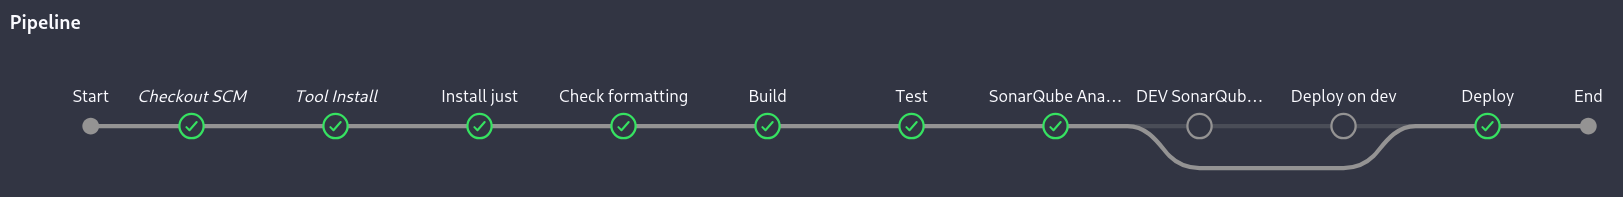
\includegraphics[width=1\textwidth]{report-jk_pipeline}
    \caption{Pipeline di Jenkins: viene lanciata a ogni evento push su GitLab e controlla formattazione, build e test; sui 
    commit delle branch \textit{main} e \textit{develop} viene anche eseguito il controllo statico del codice con SonarQube 
    e il deploy sul relativo server, di produzione o di sviluppo.}
    \label{fig:jk_pipeline}
\end{figure}

\subsubsection{SonarQube}
Come descritto nella Sezione \ref{sec:sq}, SonarQube è stato utilizzato per l'analisi della qualità del codice. Il team ha 
configurato SonarQube per eseguire analisi statiche e rilevare eventuali problematiche riguardanti la qualità del codice, 
la copertura dei test e la manutenzione.

SonarQube self-hosted è accessibile all'indirizzo \href{https://sonarqube.vezgammon.it}{\texttt{sonarqube.vezgammon.it}}

\newpage

\subsubsection{Swagger}

Per la documentazione delle API implementate e il testing più rapido, il team ha scelto di utilizzare il tool 
\textit{Swagger}(\url{https://swagger.io/}).

Vengono di seguito riportate alcune immagini che ne illustrano il funzionamento.

\begin{figure}[H]
    \centering
    \begin{minipage}[t]{0.48\textwidth}
        \centering
        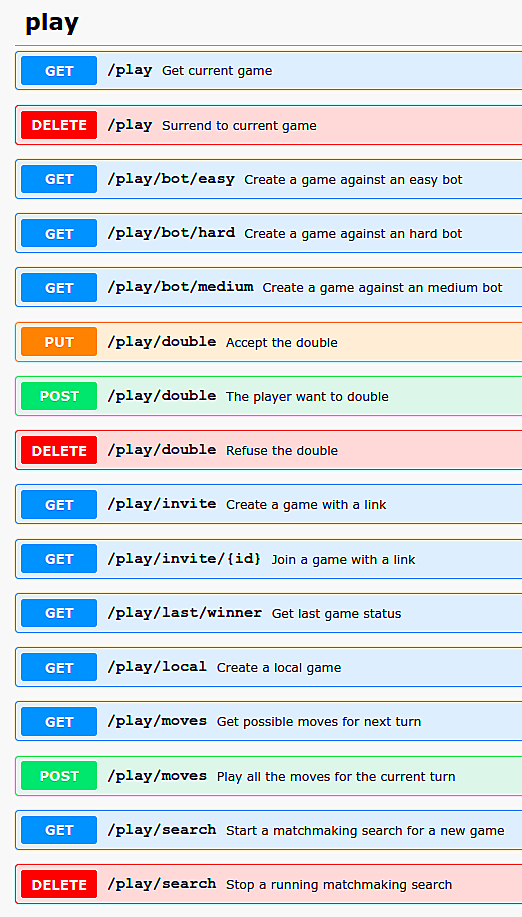
\includegraphics[width=\textwidth]{report-sw_overview}
        \caption{API utilizzate per gestire una generica partita}
        \label{fig:sw_overview}
    \end{minipage}
    \hfill
    \begin{minipage}[t]{0.49\textwidth}
        \centering
        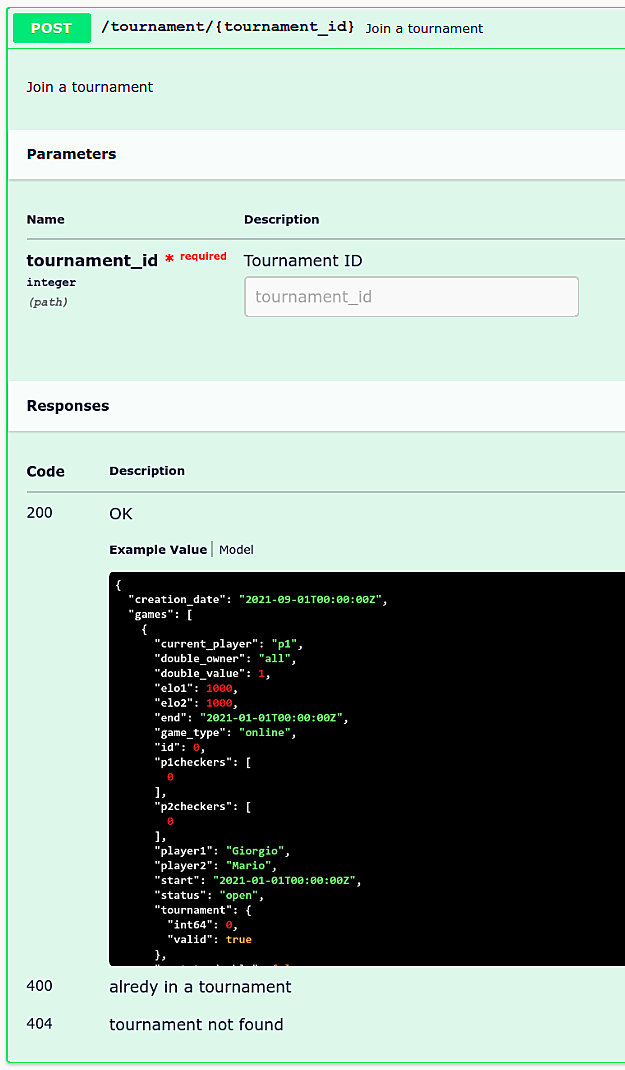
\includegraphics[width=\textwidth]{report-sw_joinTournament}
        \caption{Nel dettaglio, l'interfaccia di Swagger per ogni API}
        \label{fig:sw_joinTournament}
    \end{minipage}    
\end{figure}


\subsubsection{Status}
\label{sec:status}
Il sistema di monitoraggio dei servizi è stato sviluppato per tenere traccia della disponibilità dei vari strumenti 
utilizzati nel progetto.

\'E stato inoltre sviluppato un bot Telegram per avvisare tempestivamente il team di eventuali problemi con il server 
e/o i singoli servizi.

Il sito che riassume lo stato dei servizi è accessibile all'indirizzo \href{https://status.vezgammon.it}{\texttt{status.vezgammon.it}}

\subsection{Server di deploy}

Il team ha configurato due server principali per ospitare l'applicazione:
\begin{itemize}
    \item \textbf{Server di produzione}: \href{https://vezgammon.it}{\texttt{vezgammon.it}}
    \item \textbf{Server di sviluppo}: \href{https://dev.vezgammon.it}{\texttt{dev.vezgammon.it}}
\end{itemize}
Il server di produzione è stato utilizzato per la versione stabile, mentre il server di sviluppo è stato dedicato al testing, 
al debug e alle fasi di sviluppo continuo.


\section{Processo Scrum}
TODO MANCA SOLO QUESTO

\subsection{Sprint 0}
Oltre alle attività di teambuilding (vedi \ref{sec:teambuilding}), i membri del gruppo hanno iniziato in questa fase a studiare
il funzionamento e la documentazione dei software 

\subsection{Sprint 1}

\subsubsection{Goal}

\subsubsection{Backlog}
\begin{figure}[H]
    \centering
    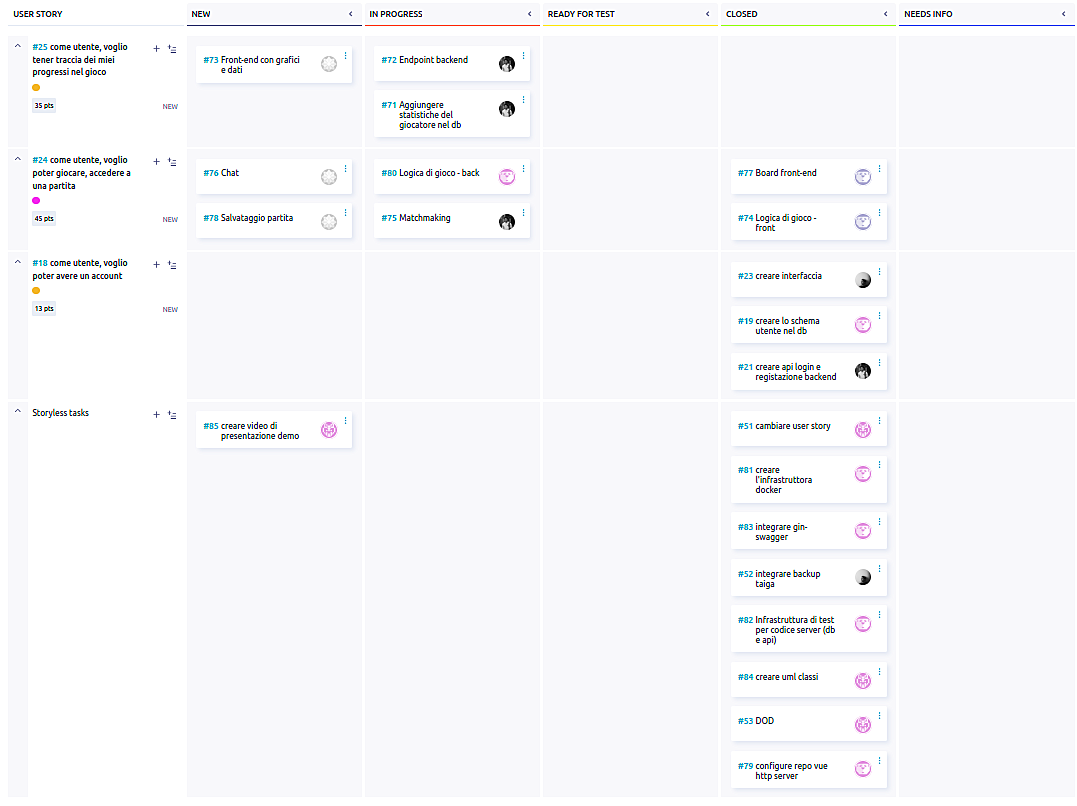
\includegraphics[width=1\textwidth]{backlog1}
    \caption{Backlog del primo sprint}
    \label{fig:backlog-s1}
\end{figure}

\subsubsection{Incremento}

\subsubsection{Definition of Done}

\subsubsection{Esempio di test fatti}

\subsubsection{Burndown}
\begin{figure}[H]
    \centering
    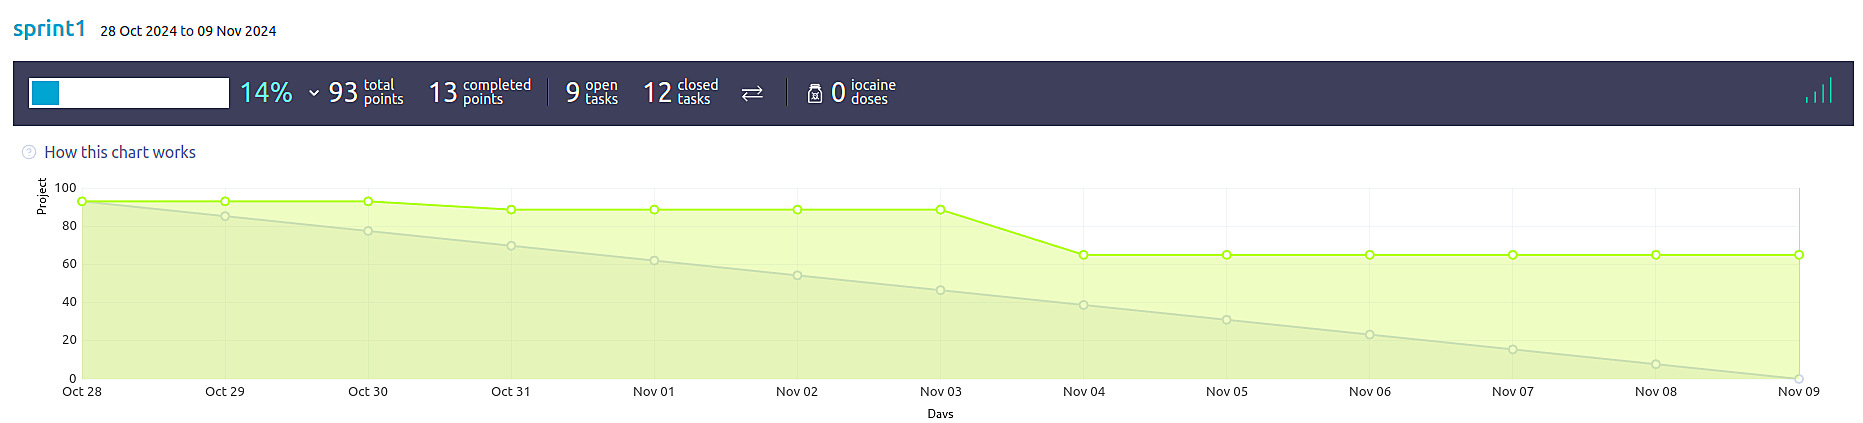
\includegraphics[width=1\textwidth]{burndown1}
    \caption{Burndown del primo sprint}
    \label{fig:burndown1}
\end{figure}

\subsubsection{Retrospettiva}

\subsection{Sprint 2}

\subsubsection{Goal}

\subsubsection{Backlog}
\begin{figure}[H]
    \centering
    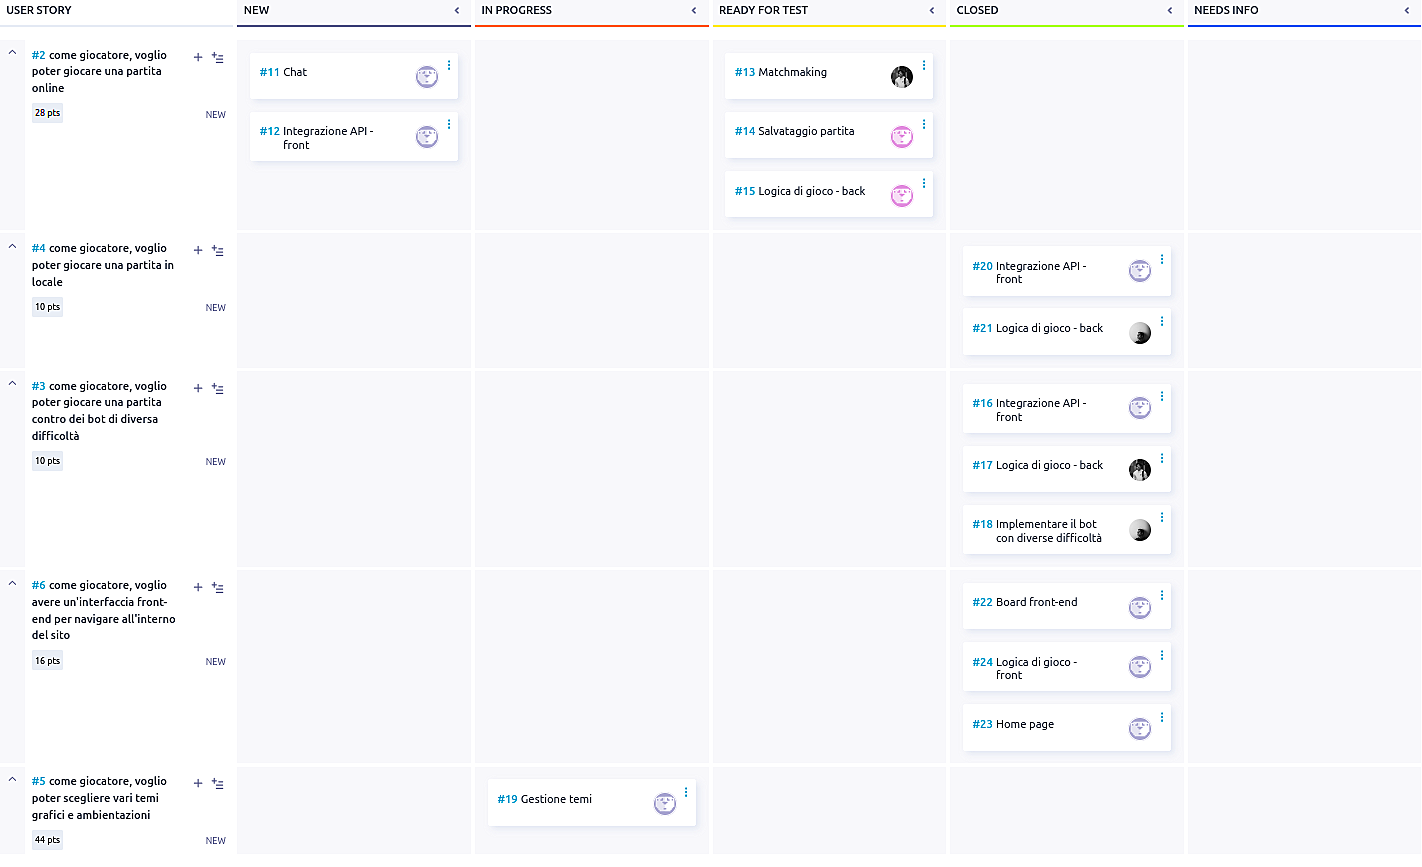
\includegraphics[width=1\textwidth]{backlog2_1}
    \caption{Backlog del secondo sprint - parte 1}
    \label{fig:backlog2_1}
\end{figure}

\begin{figure}[H]
    \centering
    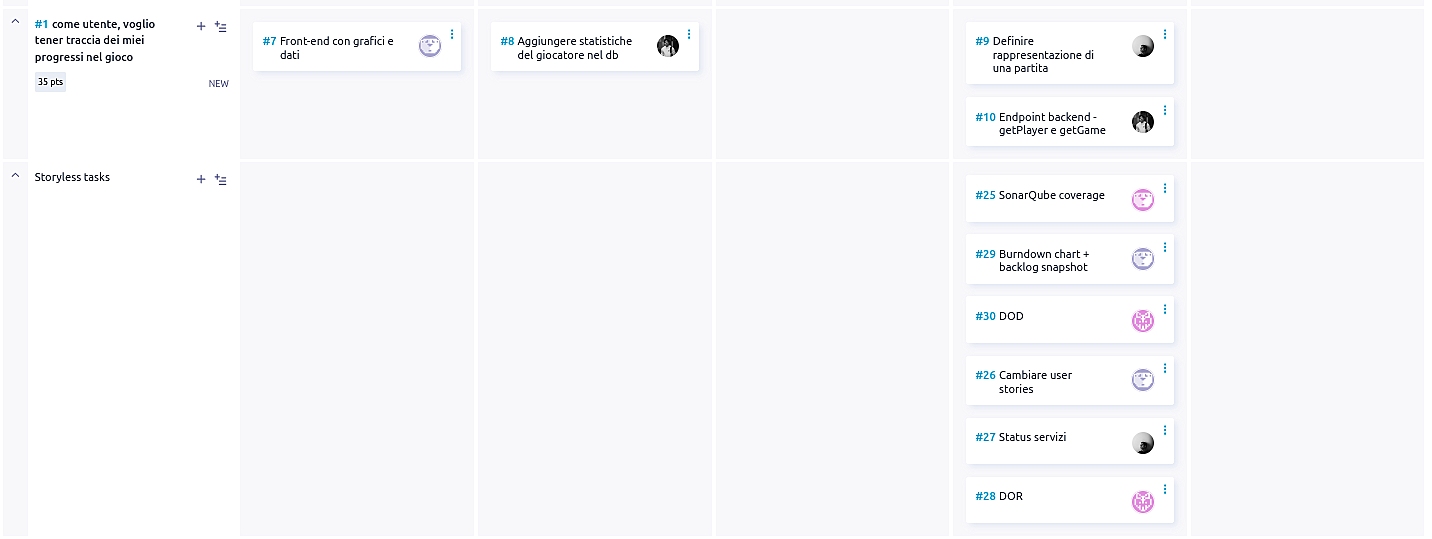
\includegraphics[width=1\textwidth]{backlog2_2}
    \caption{Backlog del secondo sprint - parte 2}
    \label{fig:backlog2}
\end{figure}

Purtroppo l'immagine originale era molto sfocata, quindi ho riprodotto il progetto di Taiga per fare questi screenshots.
Per questo motivo i numeri sulle user stories e sui task non coincidono con quelli delle altre immagini.

\subsubsection{Incremento}

\subsubsection{Definition of Done}

\subsubsection{Esempio di test fatti}

\subsubsection{Burndown}
\begin{figure}[H]
    \centering
    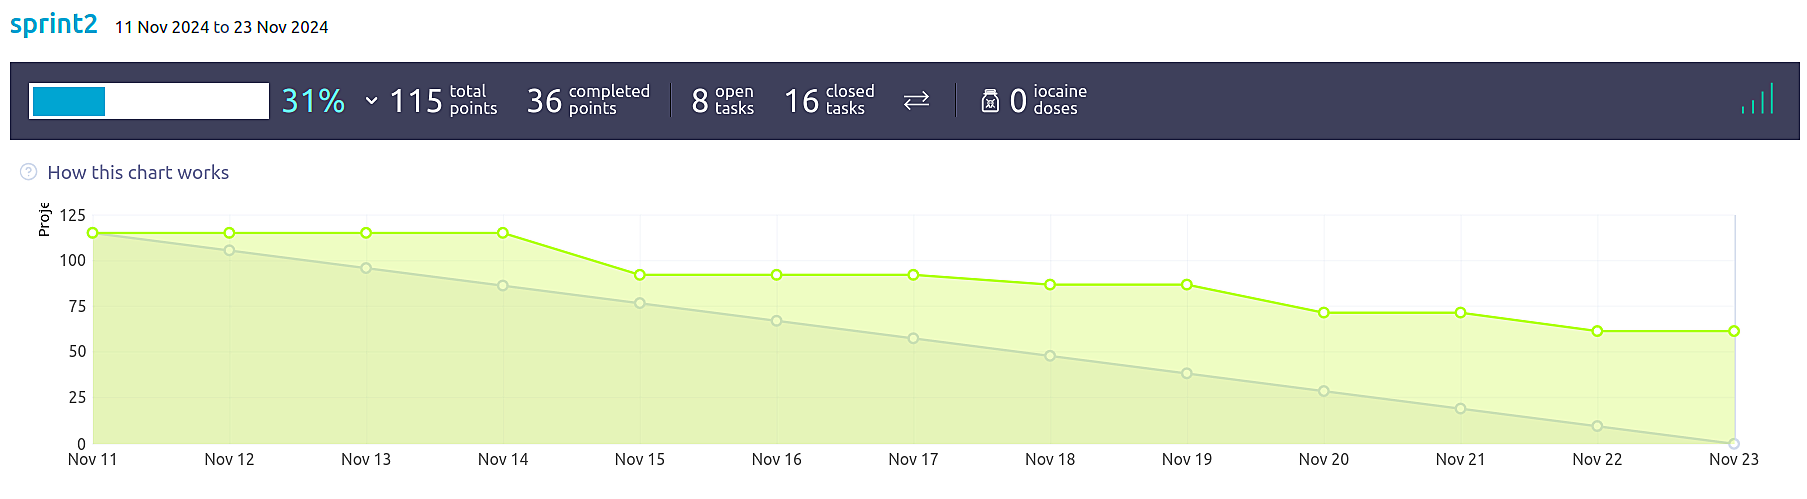
\includegraphics[width=1\textwidth]{burndown2}
    \caption{Burndown del secondo sprint}
    \label{fig:burndown2}
\end{figure}

\subsubsection{Retrospettiva}

\subsection{Sprint 3}

\subsubsection{Goal}

\subsubsection{Backlog}
\begin{figure}[H]
    \centering
    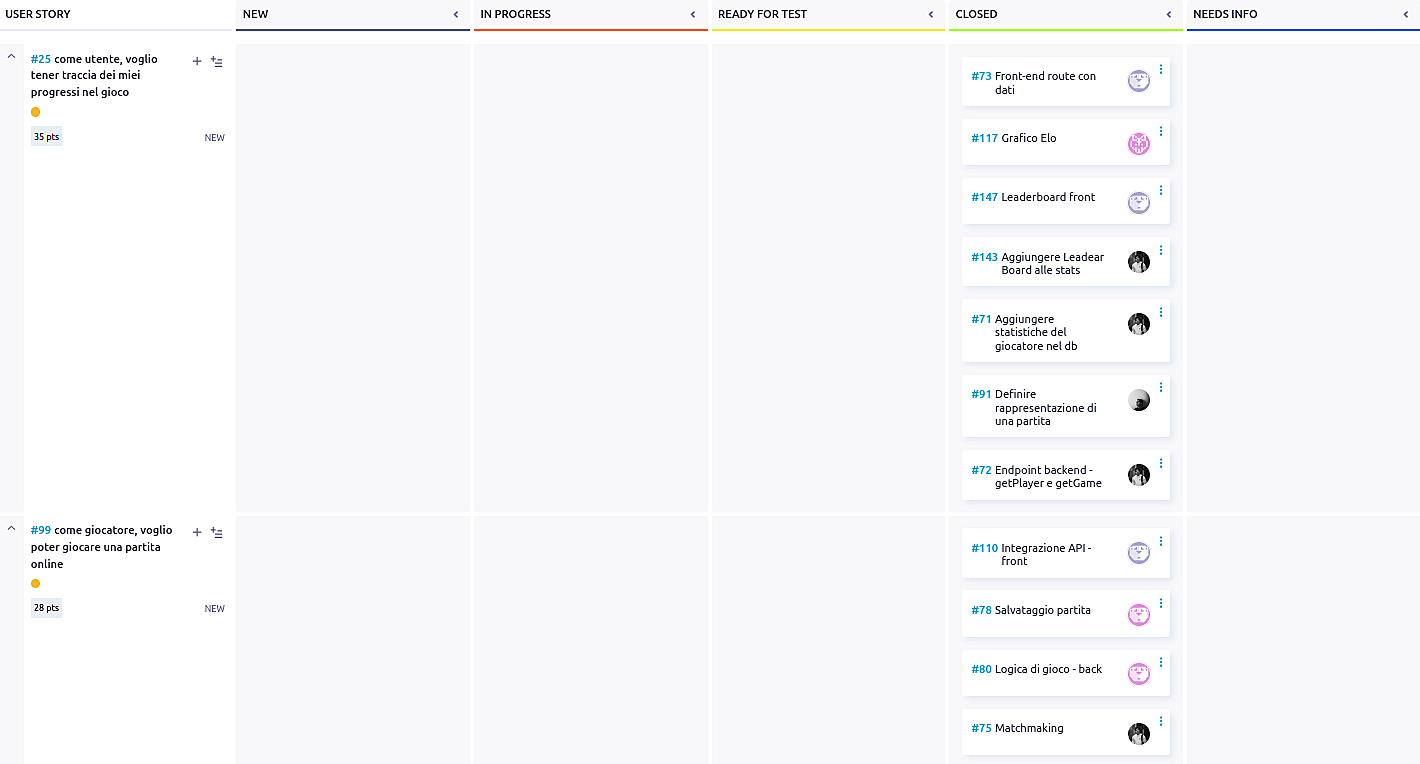
\includegraphics[width=1\textwidth]{backlog3_1}
    \caption{Backlog del terzo sprint - parte 1}
    \label{fig:backlog3_1}
\end{figure}

\begin{figure}[H]
    \centering
    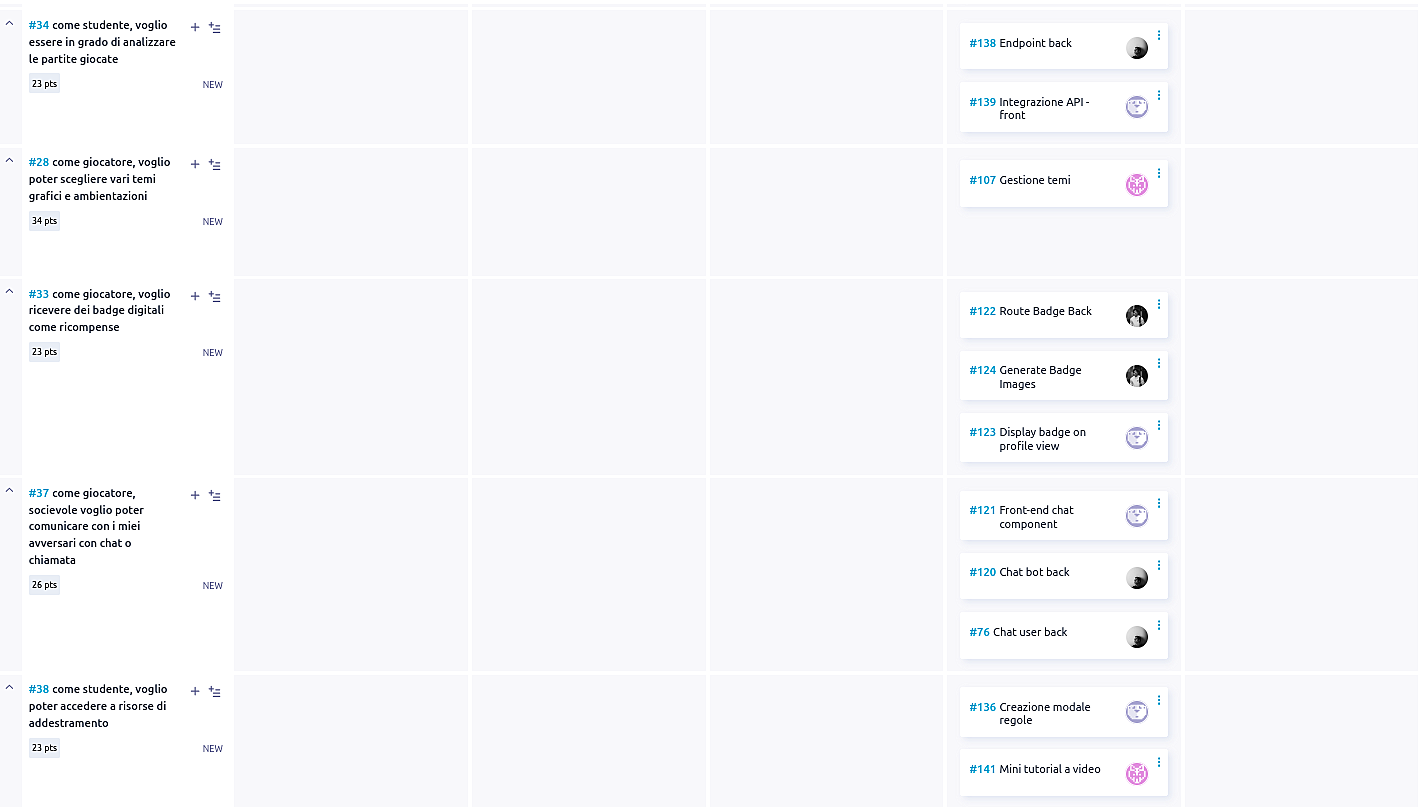
\includegraphics[width=1\textwidth]{backlog3_2}
    \caption{Backlog del terzo sprint - parte 2}
    \label{fig:backlog3_2}
\end{figure}

\begin{figure}[H]
    \centering
    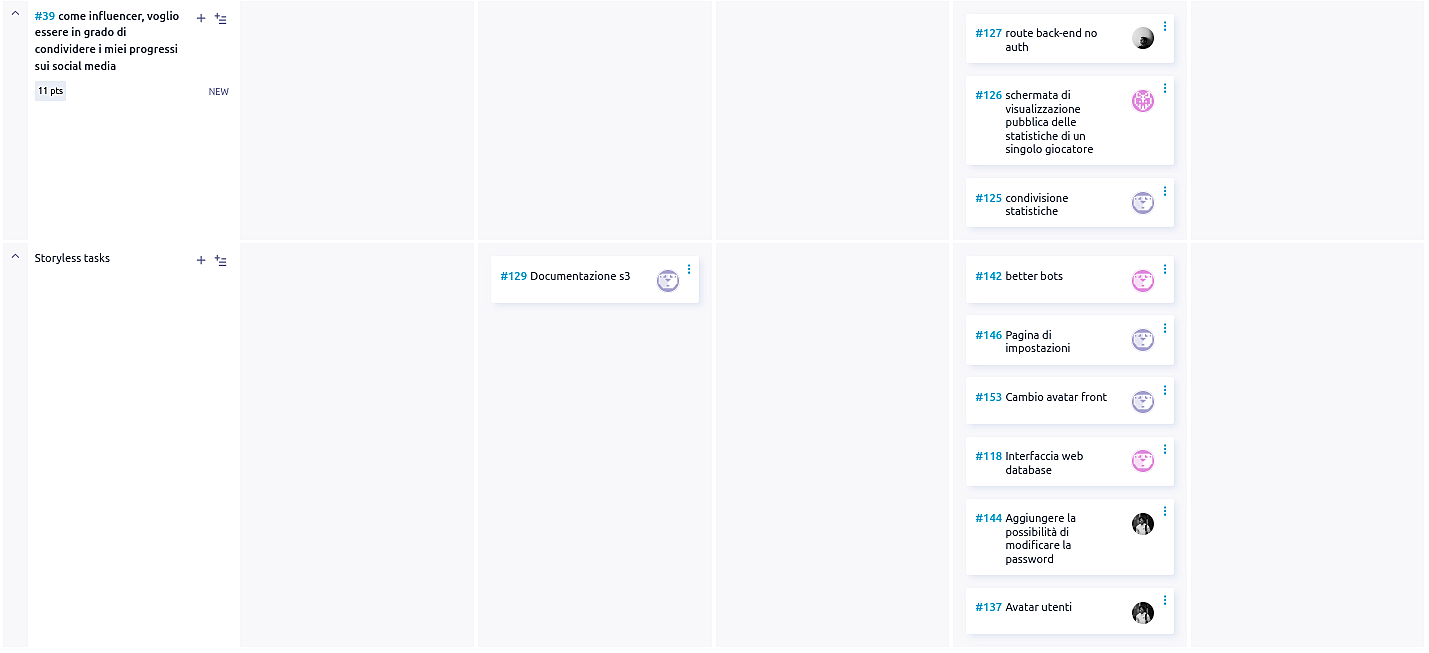
\includegraphics[width=1\textwidth]{backlog3_3}
    \caption{Backlog del terzo sprint - parte 3}
    \label{fig:backlog3_3}
\end{figure}

\subsubsection{Incremento}

\subsubsection{Definition of Done}

\subsubsection{Esempio di test fatti}

\subsubsection{Burndown}
\begin{figure}[H]
    \centering
    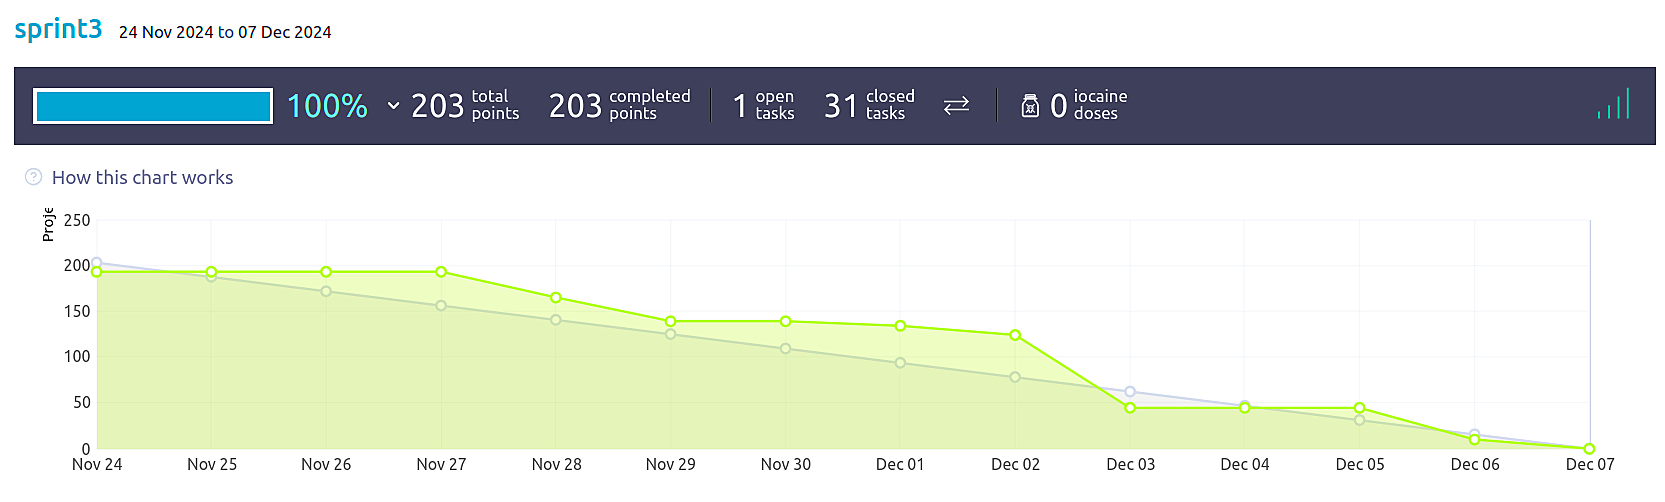
\includegraphics[width=1\textwidth]{burndown3}
    \caption{Burndown del terzo sprint}
    \label{fig:burndown3}
\end{figure}

\subsubsection{Retrospettiva}

\subsection{Sprint 4}

\subsubsection{Goal}

\subsubsection{Backlog}
\begin{figure}[H]
    \centering
    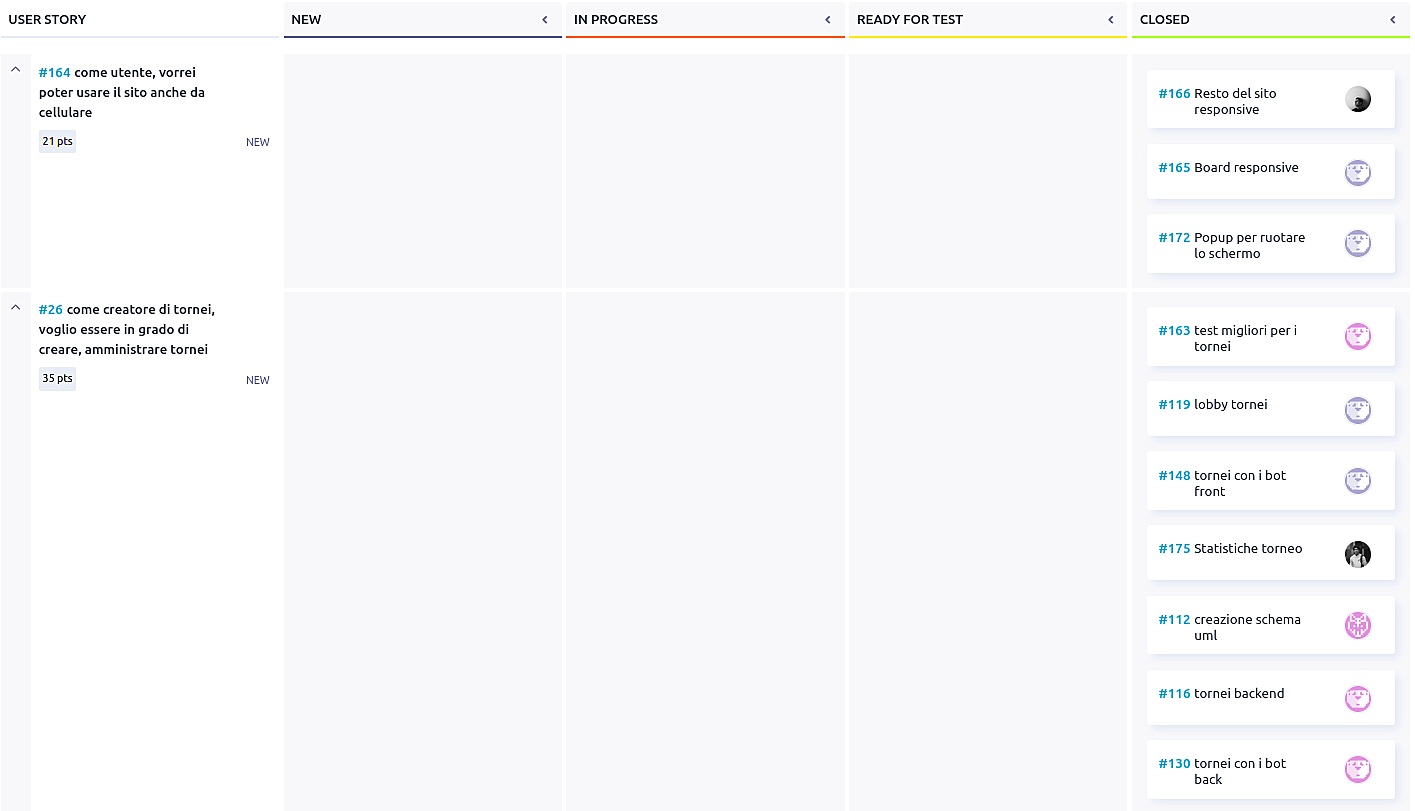
\includegraphics[width=1\textwidth]{backlog4_1}
    \caption{Backlog del quarto sprint - parte 1}
    \label{fig:backlog4_1}
\end{figure}

\begin{figure}[H]
    \centering
    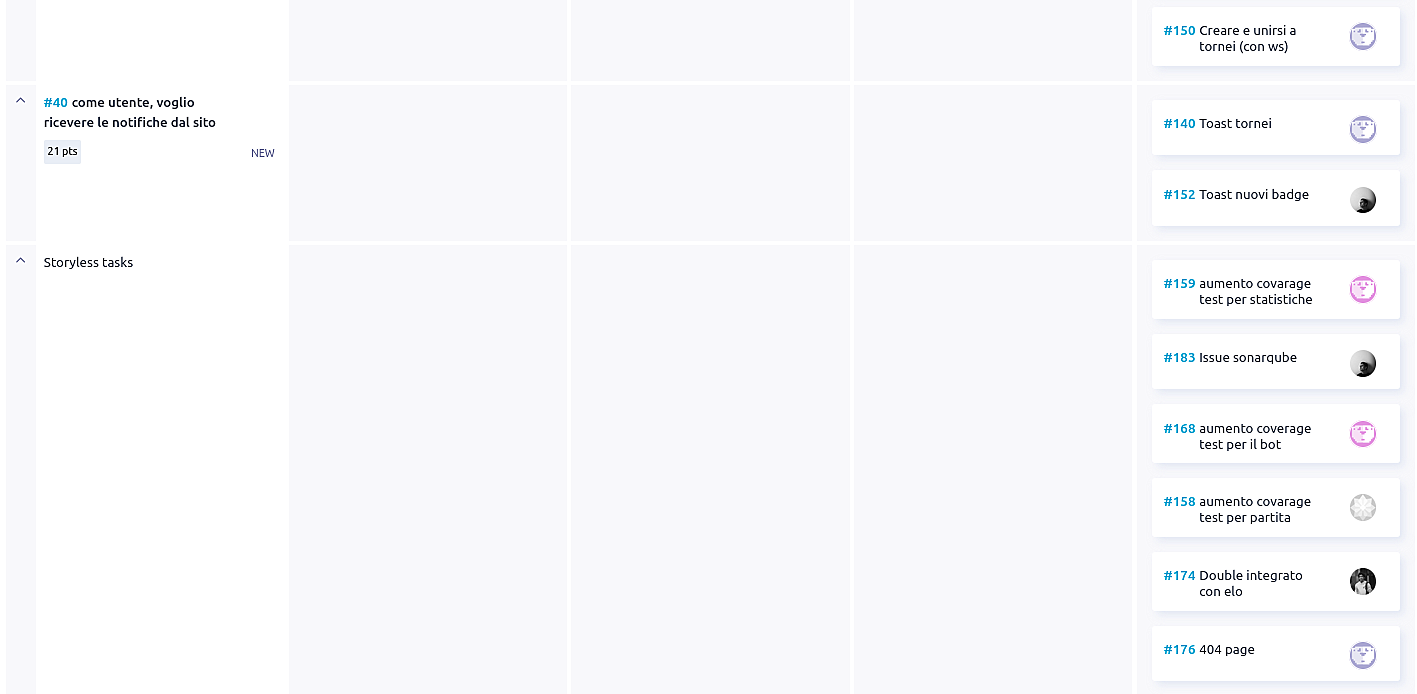
\includegraphics[width=1\textwidth]{backlog4_2}
    \caption{Backlog del quarto sprint - parte 2}
    \label{fig:backlog4_2}
\end{figure}

\subsubsection{Incremento}

\subsubsection{Definition of Done}

\subsubsection{Esempio di test fatti}

\subsubsection{Burndown}
\begin{figure}[H]
    \centering
    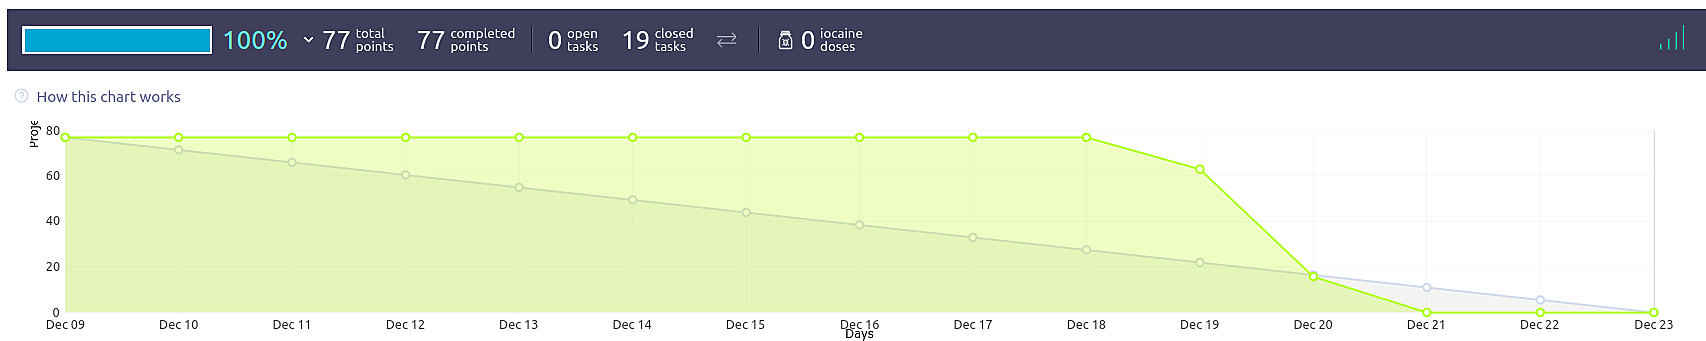
\includegraphics[width=1\textwidth]{burndown4}
    \caption{Burndown del quarto sprint}
    \label{fig:burndown4}
\end{figure}

\subsubsection{Retrospettiva}

\subsection{Release sprint}

\section{Descrizione del processo}

Il team ha deciso di comune accordo e su richiesta del \textit{Product Owner} di dedicare al progetto quattro sprint di due settimane 
ciascuno, in aggiunta allo sprint 0, dedicato alle attività di teambuilding e alla familiarizzazione con l'ambiente di sviluppo, e 
al release sprint, in cui il focus è andato sulla risoluzione dei bug, qualità del codice e stesura di questo report finale.

\subsection{Il team}

\begin{itemize}
    \item \textbf{Product Owner}: Diego Barbieri
    \item \textbf{Scrum Master}: Lorenzo Peronese
    \item \textbf{DevOps}: Samuele Musiani
    \item \textbf{Developer frontend}: Emanuele Argonni
    \item \textbf{Developer backend}: Fabio Murer
    \item \textbf{Developer backend}: Omar Ayache
\end{itemize}

Il team è composto da sei membri ed è la prima volta che lavoriamo tutti insieme su un progetto di questa portata. Sebbene non ci 
conoscessimo tutti a vicenda inizialmente, alcuni di noi avevano già collaborato durante precedenti attività, sia universitarie 
che non. Durante gli sprint abbiamo avuto modo di approfondire la conoscenza reciproca in un contesto diverso dal solito, rafforzando 
il rapporto e favorendo una collaborazione più efficace.

Prima di iniziare lo sprint 0, il team si è riunito di persona per definire i ruoli; questi sono stati rispettati per la maggior parte, 
ma con un approccio flessibile: lo Scrum Master e il Product Owner hanno aiutato nello sviluppo del frontend, mentre il DevOps ha supportato 
sia il frontend che il backend quando necessario. Questa versatilità si è rivelata vincente e ha permesso di ottimizzare il lavoro e 
affrontare le sfide che si sono presentate in modo più efficace.

\subsection{Teambuilding} \label{sec:teambuilding}

Per lo sprint 0 il team si è riunito in due giornate diverse per partecipare alle due attività di teambuilding: \textit{Scrumble} e 
\textit{Escape The Boom!}.

Il primo gioco, \textit{Scrumble}, si è rivelato inizialmente complicato da comprendere; tuttavia, una volta avviata l'attività, i membri 
del team hanno rapidamente preso il ritmo. Nonostante gli obiettivi prefissati del gioco non siano stati minimamente raggiunti, l'esperienza 
si è rivelata piacevole e coinvolgente. Il team ha avuto l'opportunità di familiarizzare con la metodologia Scrum, un "assaggio" pratico 
di come funziona il lavoro in sprint.

Il secondo gioco, \textit{Escape The Boom!}, è stato più intuitivo da avviare ma non meno impegnativo. Il team si è suddiviso in due gruppi: 
il primo era incaricato di leggere e interpretare le istruzioni, mentre il secondo aveva il compito di disinnescare la bomba virtuale. Anche 
in questo caso, il gruppo ha trascorso un'ora divertente e stimolante, sebbene con risultati altrettanto modesti.

Di seguito la tabella dell'autovalutazione di \textit{Scrumble}, compilata da tutti i partecipanti:

\begin{figure}[H]
    \centering
    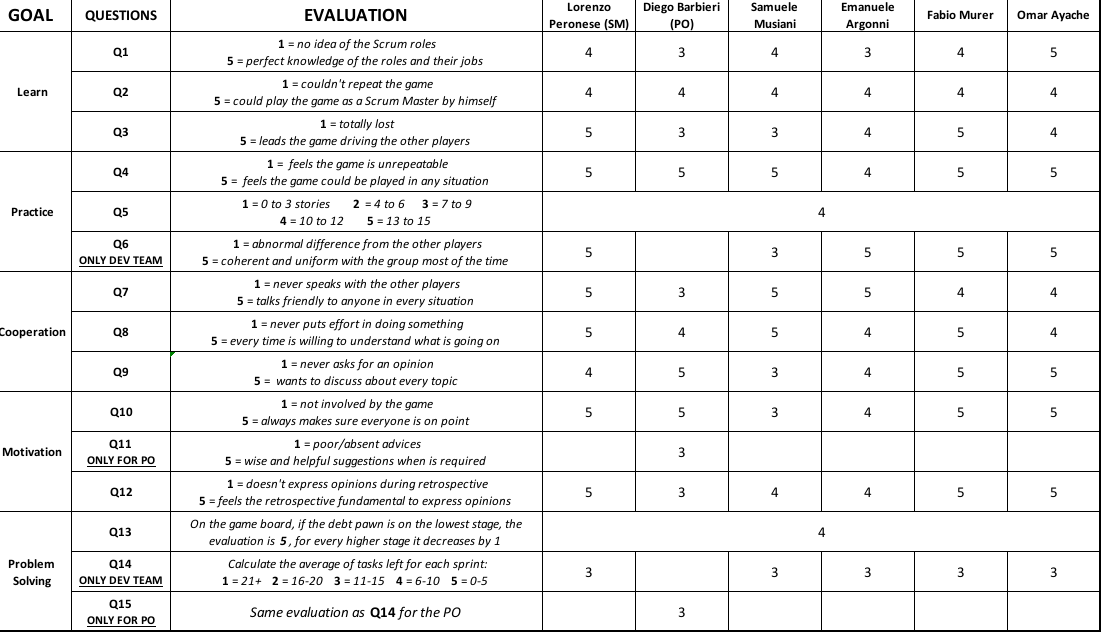
\includegraphics[width=1\textwidth]{report-scrumble}
    \caption{Tabella di autovalutazione del gioco \textit{Scrumble}}
    \label{fig:scrumble}
\end{figure}


\subsection{Gitinspector}

Le statistiche fornite dal Professor/Stakeholder Missiroli, generate tramite Gitinspector, non risultano essere accurate (il numero di commit 
segnalato da Gitinspector è di molto inferiore al numero reale). Non siamo riusciti a determinare con certezza se il problema risieda nel nostro 
repository o nel software stesso. Tuttavia, dopo aver effettuato ulteriori analisi indipendenti utilizzando Gitinspector, abbiamo riscontrato 
gli stessi risultati non corretti. Per completezza, i dati originali sono disponibili su 
\href{https://gitlab.vezgammon.it/diego/vezgammon/-/tree/main/doc/feedback_stakeholders}{\texttt{GitLab}}.

In questo report, vengono confivise invece le statistiche del repository ottenute tramite 
\href{https://github.com/git-quick-stats/git-quick-stats}{\texttt{git-quick-stats}}, un altro strumento di analisi. 

Si segnala che i dati riportati non includono la stesura di questo documento.

\begin{figure}[H] 
    \centering 
    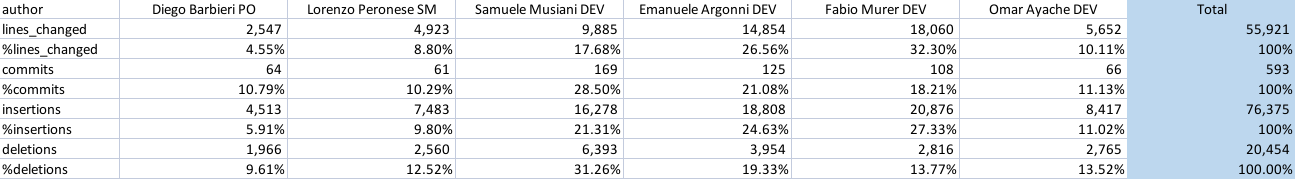
\includegraphics[width=\textwidth]{report-stats_raw} 
    \caption{Dati grezzi ricavati da git-quick-stats} 
    \label{fig:stats_raw} 
\end{figure}

\begin{figure}[H] 
    \centering 
    \begin{minipage}[t]{0.44\textwidth} 
        \centering 
        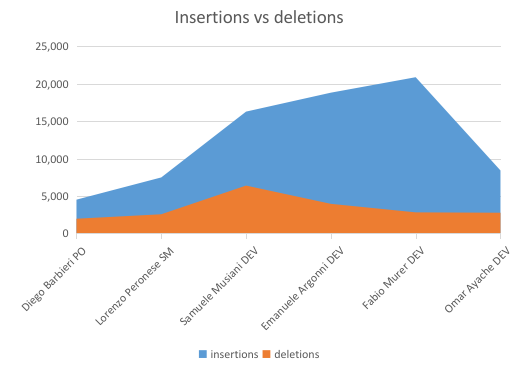
\includegraphics[width=\textwidth]{report-stats_insdel} 
        \caption{Rapporto tra linee inserite ed eliminate, le righe persistenti complessive sono oltre 55 mila} 
        \label{fig:stats_insdel} 
    \end{minipage} 
    \hfill 
    \begin{minipage}[t]{0.51\textwidth} 
        \centering 
        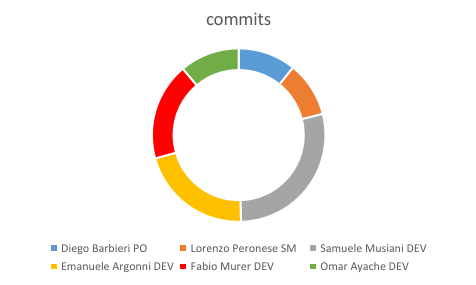
\includegraphics[width=\textwidth]{report-stats_commits} 
        \caption{Numero di commit nel repository, per un totale di 593 e una media di circa 15 al giorno} 
        \label{fig:stats_commits} 
    \end{minipage}
\end{figure}

\subsection{Monitoraggio delle ore}
Per il monitoraggio delle ore spese nel progetto non abbiamo utilizzato software di logging. Questa scelta è stata motivata dalla diversità di 
IDE utilizzati dai membri del team, che ha reso difficile individuare uno strumento compatibile per tutti. Inoltre, abbiamo provato inizialmente 
a utilizzare un timer per tracciare le ore, ma ci siamo resi conto che, non essendo un lavoro a tempo pieno, era comune dedicarsi ad altre 
attività durante le sessioni di scrittura del codice, questo rendeva il timer uno strumento poco adatto alla nostra situazione.

Abbiamo quindi optato per un approccio più semplice e flessibile, utilizzando un foglio Excel condiviso. Ogni membro del team ha segnato manualmente 
le ore effettivamente dedicate al progetto, garantendo una panoramica chiara e trasparente del tempo complessivamente investito. Di seguito quindi 
la tabella appena citata.

\begin{figure}[H]
    \centering
    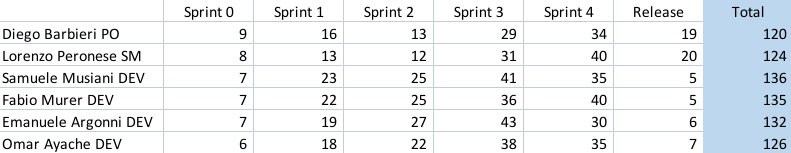
\includegraphics[width=1\textwidth]{report-logging_raw}
    \caption{Dati grezzi raccolti durante lo sviluppo}
    \label{fig:logging}
\end{figure}

\begin{figure}[H]
    \centering
    \begin{minipage}[t]{0.52\textwidth}
        \centering
        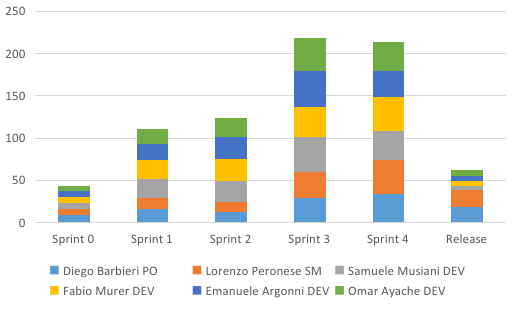
\includegraphics[width=\textwidth]{report-logging_sprints}
        \caption{Ore di lavoro per ogni sprint, il totale è 773 ore (32 interi giorni!)}
        \label{fig:logging-sprints}
    \end{minipage}
    \hfill
    \begin{minipage}[t]{0.47\textwidth}
        \centering
        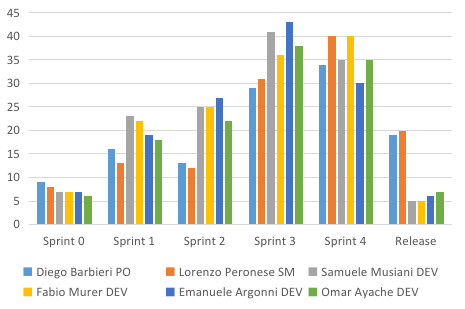
\includegraphics[width=\textwidth]{report-logging_full}
        \caption{Più nel dettaglio, ore di lavoro per membro del team per sprint}
        \label{fig:logging-full}
    \end{minipage}    
\end{figure}



\subsection{Strumenti di comunicazione} \label{sec:mm}
Per comunicare tra noi abbiamo deciso di usare MatterMost, una piattaforma di chat e condivisione interamente open-source. Come per gli altri 
servizi, anche MatterMost è stato self-hostato sotto il dominio vezgammon.it per avere un maggiore controllo sui dati. Questa scelta ha permesso 
al team di gestire in autonomia l'infrastruttura di comunicazione, evitando dipendenze da servizi esterni e assicurando la personalizzazione 
dell'ambiente in base alle necessità del progetto.

MatterMost è stato utilizzato per la comunicazione quotidiana, la condivisione di aggiornamenti e l'organizzazione degli incontri di persona, 
che si sono svolti con frequenza. Gli incontri hanno avuto luogo presso il laboratorio del gruppo ADMstaff, situato nel seminterrato del 
Dipartimento di Informatica, in Mura Anteo Zamboni 7.

Il laboratorio è diventato il punto di riferimento per il team, che vi si è riunito interi pomeriggi per daily scrum, sessioni di pair programming 
e discussioni sull'avanzamento generale del progetto. Questa modalità di lavoro ha favorito una collaborazione continua e diretta, contribuendo 
significativamente alla coesione del gruppo e al progresso del progetto.

Come strumento di comunicazione secondario è stato usato Telegram per comunicazioni meno "ufficiali" e sopratutto per ricevere notifiche relative 
allo stato dei vari servizi tramite \textit{Status} (vedi \ref{sec:status}).

\subsection{Utilizzo di Large Language Models}

Abbiamo integrato strategicamente diversi modelli di intelligenza artificiale generativa nello sviluppo del progetto. Nello specifico, abbiamo 
impiegato GitHub Copilot per l'autocompletamento del codice ripetitivo direttamente nell'IDE, Claude per la risoluzione di problematiche tecniche 
specifiche e ChatGPT per la stesura della documentazione.

L'approccio all'utilizzo di questi strumenti è stato mirato: per ogni problema, abbiamo scelto di impiegare l'AI o come supporto iniziale 
nell'esplorazione delle possibili soluzioni o come strumento per risolvere un particolare problema o perfezionare un'implementazione già esistente, 
evitando la sovrapposizione dei due metodi.

Nonostante questi strumenti abbiano contribuito a incrementare la produttività del team, il loro impiego ha richiesto particolare attenzione: le 
"allucinazioni" e gli errori nel codice generato hanno reso necessaria un'attenta verifica delle risposte e in diverse occasioni il tempo dedicato 
al debugging del codice generato ha superato il risparmio di tempo ottenuto nella sua scrittura.

Con l'esperienza, siamo giunti a un equilibrio efficace che ci ha permesso di sfruttare le potenzialità di questi potenti strumenti mantenendo al 
contempo un controllo adeguato per cercare di arginarne i lati negativi.

\subsubsection{Esempi di Prompt Utilizzati}

Di seguito sono riportati alcuni esempi a titolo esemplificativo dei prompt utilizzati, organizzati per categoria: \\ \\
\begin{tabular}{>{\columncolor{blue!30}}p{0.0001\textwidth} p{1\textwidth}}
    & - Fix this vue component error: \texttt{\{...\}} \\
    & - How do I refactor the code to make it work with tailwind themes? \\
\end{tabular}
\begin{tabular}{>{\columncolor{green!30}}p{0.0001\textwidth} p{1\textwidth}}
    & - Given these SQL tables: \texttt{\{...\}} Make a SQL query to return the table \texttt{game} with usernames instead of \texttt{p1\_id}, \texttt{p2\_id}. \\
    & - PostgreSQL returns error: \texttt{syntax error at or near "FROM"} for the following query: \texttt{\{...\}} \\
\end{tabular}
\begin{tabular}{>{\columncolor{red!30}}p{0.0001\textwidth} p{1\textwidth}}
    & - Reformulate this user story: \texttt{\{...\}} Make it detailed enough for developers but not too technical for the client. \\
    & - This user story is too challenging: \texttt{\{...\}} Break it down into 3/4 smaller and more manageable user stories. \\
\end{tabular}
\begin{tabular}{>{\columncolor{orange!30}}p{0.0001\textwidth} p{1\textwidth}}
    & - How can I make this retrospective more objective and data-based? \texttt{\{...\}} \\
    & - How can I make this documentation more concise while maintaining all essential information? \texttt{\{...\}} \\
\end{tabular}

\subsection{SonarQube} \label{sec:sq}

\begin{figure}[H]
    \centering
    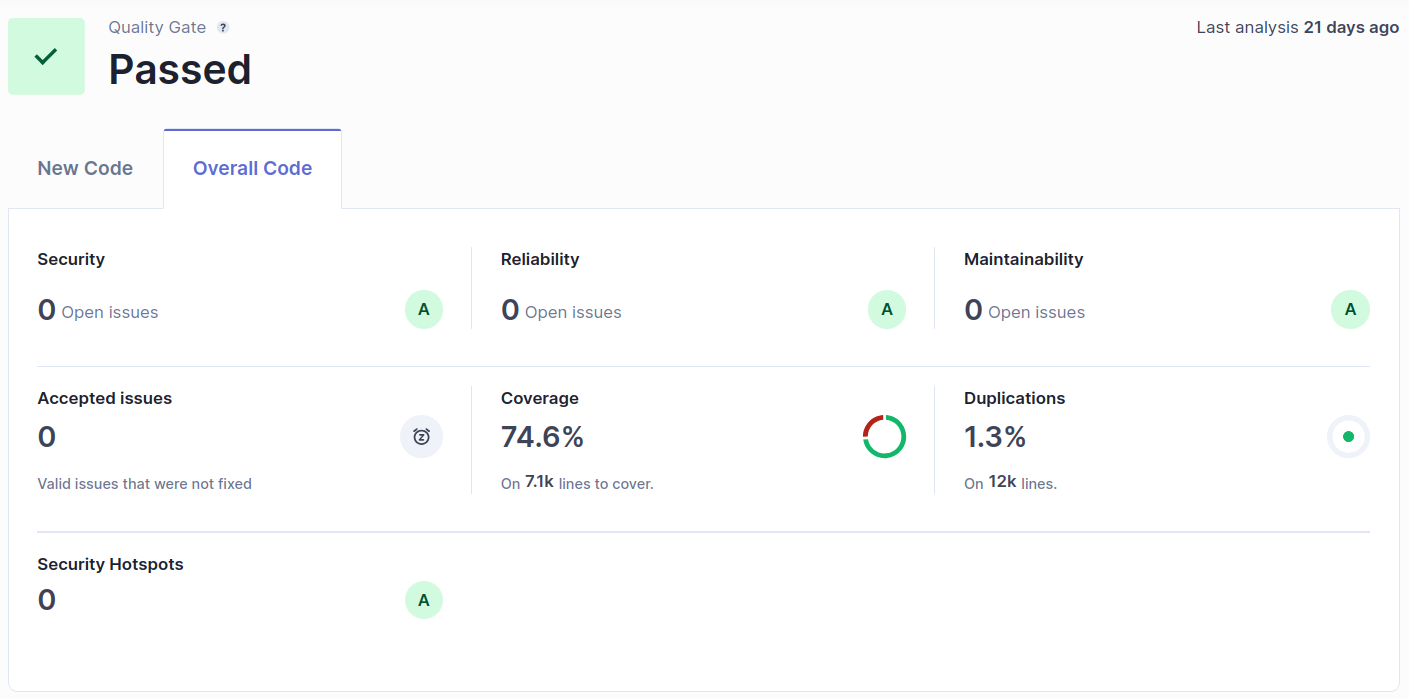
\includegraphics[width=1\textwidth]{report-sq_overview}
    \caption{Vista generale di SonarQube, che mostra un riepilogo delle metriche del progetto, tra cui copertura del codice, vulnerabilità, codice duplicato 
    e molto altro. \\
    L'obiettivo di una copertura del 50\% è stato abbondantemente superato; tuttavia le aree di codice meno coperte dai test riguardano principalmente le API 
    e le parti che fanno uso dei web socket, in quanto più difficili da testare.}
    \label{fig:sq_overview}
\end{figure}

\begin{figure}[H]
    \centering
    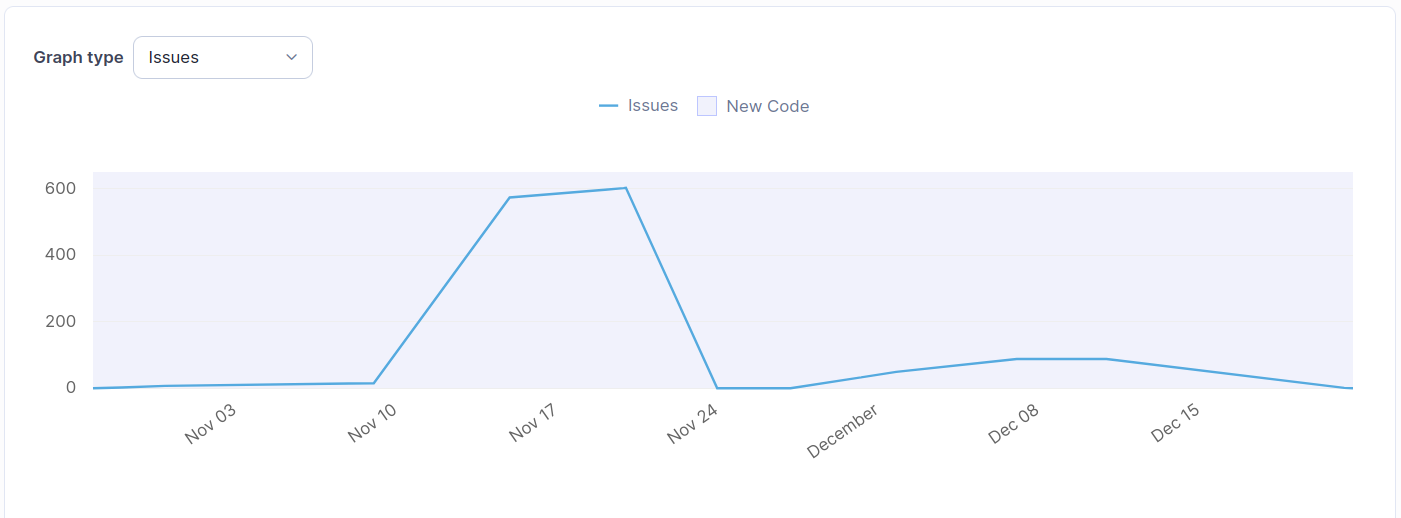
\includegraphics[width=1\textwidth]{report-sq_issues}
    \caption{Grafico delle issue rilevate nel tempo: il picco registrato intorno al 15 novembre è legato all'inclusione di due file HTML di GitInspector simili, 
    che ha portato SonarQube a rilevare numerosi problemi di duplicazione. Dopo aver individuato la causa, abbiamo escluso quei file dall'analisi, riportando 
    i valori alla normalità. Durante il resto dello sviluppo, il numero delle issue è stato mantenuto sotto controllo, risolvendo i problemi a intervalli regolari.}
    \label{fig:sq_issues}
\end{figure}


\section{Demo 3 min}
Link qui

\end{document}